\documentclass[tikz]{standalone}

\begin{document}

	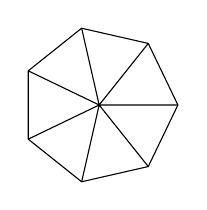
\begin{tikzpicture}
	% Define the desired points
	\coordinate (origin) at (0,0);
	\coordinate (A) at (360.0 / 7.0 * 0 : 1);
	\coordinate (B) at (360.0 / 7.0 * 1 : 1);
	\coordinate (C) at (360.0 / 7.0 * 2 : 1);
	\coordinate (D) at (360.0 / 7.0 * 3 : 1);
	\coordinate (E) at (360.0 / 7.0 * 4 : 1);
	\coordinate (F) at (360.0 / 7.0 * 5 : 1);
	\coordinate (G) at (360.0 / 7.0 * 6 : 1);
	% Draw the edges
	\draw (A) -- (B) -- (C) -- (D) -- (E) -- (F) -- (G) --cycle;
	% Add spokes
	\draw (origin) -- (A) (origin) -- (B) (origin) -- (C) (origin) -- (D) (origin) -- (E) (origin) -- (F) (origin) -- (G);
	\end{tikzpicture}
\end{document}